% =========================================================================
% Secao 7 - Robustez
% =========================================================================

\section{Robustez}
\label{sec:robustez}
\label{ssec:atrito}

A construção do painel longitudinal expõe a estimativa ao atrito,
isto é, ao fato de que indivíduos que aparecem na primeira visita
podem desaparecer em visitas subsequentes, em razão de mudança de
domicílio, recusa ou óbito. Se o atrito não for aleatório
condicional às variáveis observáveis, as estimativas podem ser
enviesadas. Sob a metodologia da Seção~\ref{ssec:definicoes}, que
restringe a janela de transição a $Q_2$ e $Q_3$, há atrito de dois
tipos. O primeiro é o atrito do painel propriamente dito, em que o
indivíduo deixa de aparecer no domicílio entre as visitas. O segundo
é o atrito estrutural decorrente da restrição $Q_2$--$Q_3$, em que
apenas domicílios que entram no painel em $Q_2$ ou $Q_3$ do ano $t$
contribuem para a transição $t \to t+1$, o que corresponde a cerca
de quarenta por cento da amostra total e impõe redução substancial
de tamanho amostral.

Para o atrito de painel, no painel construído, 1.731.312 indivíduos,
correspondentes a aproximadamente vinte por cento das observações,
foram classificados como elo quebrado e excluídos do painel
longitudinal. Os 6.915.911 retidos formam a base do exercício. Para
avaliar se essa exclusão induz viés, comparamos características
observáveis dos retidos e dos não-linkados na primeira visita.
Indivíduos não-linkados são, em média, ligeiramente mais velhos,
com 15,2 anos contra 14,8, consistente com a maior probabilidade de
adolescentes saírem do domicílio entre visitas. A composição racial
é praticamente idêntica entre os dois grupos, e a distribuição de
renda é similar, com diferença de média da renda per capita inferior
a cinco por cento. Implementamos a reponderação por \emph{inverse
propensity}, esquema P3 descrito no
Apêndice~\ref{app:variaveis}. Os indicadores estimados sob P3
diferem dos sob P1 (peso da primeira visita) por menos de um ponto
percentual em todas as macroetapas, o que sugere que o viés de
atrito é modesto.

Para o atrito condicional à restrição $Q_2$--$Q_3$, ressalva-se o
seguinte. Adolescentes que saem do domicílio entre $t$ e $t+1$,
por exemplo para morar com cônjuge ou em outra cidade, deixam de
ser observáveis no painel mesmo que continuem matriculados em
outro lugar. Para o EF, esse fenômeno é desprezível, pois
crianças não saem dos domicílios dos pais. Para o EM, contudo, é
potencialmente substancial. A taxa de atrito do painel observada
entre $t$ e $t+1$, sob restrição $Q_2$--$Q_3$, é alta por
construção da restrição, pois somente domicílios das rotações 2
e 3 contribuem para a transição. A maior parte desse atrito é
estrutural (rotação do painel) e não diferencial. Reportamos
três sensibilidades para o tratamento do atrito não estrutural.
Na variante \emph{drop}, padrão adotado nos números reportados
nas tabelas principais, excluímos casos de atrito. Na variante
\emph{evasão} assumimos que todos os atritados evadiram, o que
estabelece um limite superior para a evasão. Na variante
\emph{IPS}, reponderamos por \emph{inverse propensity}
condicional a idade, sexo, raça, renda e UF. Em todas as
sensibilidades, o ordenamento qualitativo entre macroetapas é
preservado, e a evasão do EM permanece próxima de seis por cento
em todas as variantes, dentro de um intervalo de plus or minus
dois pontos percentuais.

\subsection{O paradoxo COVID e a anomalia pós-pandêmica}
\label{ssec:paradoxo_covid}

Os anos a partir de 2020 apresentam um padrão paradoxal nos
indicadores de fluxo que merece discussão dedicada. Durante a
pandemia, sistemas estaduais e municipais de educação adotaram
amplamente políticas de aprovação automática ou suspensão da
reprovação. O efeito esperado seria um aumento da promoção e
uma queda da repetência. A Tabela~\ref{tab:paradoxo_covid}
mostra que essa é exatamente a leitura do registro
administrativo do INEP, mas o oposto da leitura da PNADC.

% C25 paradoxo COVID
\begin{table}[htbp]\centering
\caption{Paradoxo COVID: comparac\~ao direta entre INEP e PNADC v5 nos anos 2018--2021. Durante 2020 e 2021, o INEP registra promoc\~ao mais alta e repet\^encia mais baixa (compat\'ivel com aprovac\~ao autom\'atica), enquanto a PNADC registra o oposto.}
\label{tab:paradoxo_covid}
\begin{threeparttable}\small
\begin{tabular}{lrrrrrrrr}\toprule
& \multicolumn{2}{c}{Promo\c{c}\~ao (\%)} & \multicolumn{2}{c}{Repet\^encia (\%)} & \multicolumn{2}{c}{Evas\~ao (\%)} & \multicolumn{2}{c}{$\Delta$ prom.\ (pp)} \\
\cmidrule(lr){2-3} \cmidrule(lr){4-5} \cmidrule(lr){6-7} \cmidrule(lr){8-9}
Ano $t$ & INEP & PNADC & INEP & PNADC & INEP & PNADC & 2020/19 & 2021/19 \\
\midrule
\multicolumn{9}{l}{\textit{EF iniciais}} \\
\midrule
2018 & 92.6 & 86.3 & 6.1 & 11.7 & 1.2 & 0.4 & &  \\
2019 & 93.4 & 86.1 & 5.2 & 11.9 & 1.3 & 0.4 & &  \\
2020 & 96.2 & 76.9 & 2.2 & 21.9 & 1.5 & 0.4 & I:+2.8 P:-9.2 & \\
2021 & 95.5 & 82.9 & 3.1 & 16.0 & 1.3 & 0.2 & & I:+2.1 P:-3.2 \\
\\[0.3em]
\multicolumn{9}{l}{\textit{EF finais}} \\
\midrule
2018 & 85.0 & 81.0 & 8.8 & 13.6 & 3.9 & 2.0 & &  \\
2019 & 87.2 & 81.4 & 8.0 & 13.8 & 3.0 & 1.3 & &  \\
2020 & 93.9 & 73.1 & 2.3 & 24.7 & 2.9 & 0.8 & I:+6.7 P:-8.3 & \\
2021 & 91.2 & 80.4 & 3.3 & 15.9 & 4.0 & 2.0 & & I:+4.0 P:-1.0 \\
\\[0.3em]
\multicolumn{9}{l}{\textit{EM}} \\
\midrule
2018 & 79.5 & 75.7 & 8.2 & 13.6 & 9.7 & 7.4 & &  \\
2019 & 82.7 & 75.8 & 8.3 & 15.0 & 6.9 & 5.9 & &  \\
2020 & 89.0 & 63.5 & 3.9 & 29.9 & 5.9 & 3.8 & I:+6.3 P:-12.3 & \\
2021 & 85.3 & 73.4 & 4.2 & 17.9 & 8.7 & 6.8 & & I:+2.6 P:-2.4 \\
\bottomrule\end{tabular}
\begin{tablenotes}\footnotesize
\item \textit{Fontes:} INEP Indicadores de Trajet\'oria (Brasil) e painel longitudinal PNADC v5.
\item \textit{Notas:} ``$\Delta$ prom.\ 2020/19'' \'e a varia\c{c}\~ao da promoc\~ao em 2020 em relac\~ao a 2019, pelas duas fontes (I = INEP, P = PNADC). Sinais opostos entre INEP e PNADC indicam que as duas fontes capturam dimens\~oes distintas do mesmo fen\^omeno: registro administrativo de matr\'icula vs.\ auto-relato familiar sobre a situac\~ao escolar.
\end{tablenotes}\end{threeparttable}\end{table}


No ensino médio, a transição 2019/2020 reportada pelo INEP
mostra promoção saltando de 82,7\% para 89,0\% e repetência
caindo de 8,3\% para 3,9\%. A PNADC mostra o oposto. A
promoção no EM cai de 75,8\% em 2019 para 63,5\% em 2020, ao
passo que a repetência sobe de 15,0\% para 29,9\%, quase
dobrando. A explicação mais plausível para essa divergência
em 2020 é a defasagem entre a situação administrativa
registrada pela instituição e o auto-relato familiar coletado
pela PNADC. Com escolas fechadas, comunicação institucional
prejudicada e calendário letivo bagunçado, é plausível que
muitas famílias não tenham sido informadas sobre a promoção
automática do aluno, ou não tenham compreendido que ela teria
ocorrido, e continuaram reportando à PNADC a série que o
aluno cursava no início da pandemia.

O dado mais intrigante, contudo, não é o que acontece em 2020.
É o que acontece em 2022 e 2023. Em 2021, a repetência no EM
voltou a 17,9\%, próxima do nível pré-pandêmico, sugerindo que
a confusão de auto-relato seria temporária e estaria se
dissipando. Em 2022 e 2023, contudo, a repetência subiu
novamente para 27,6\% e 28,3\%, valores quase duas vezes
maiores que o pré-pandemia. O padrão se manifesta de forma
sistemática em todos os níveis do EM. Entre alunos no 1º ano
do EM que estavam matriculados em $t+1$, a proporção
reportada na mesma série era de 17,7\% em 2019, saltou para
30,2\% em 2022 e mantém-se nesse patamar em 2023. No 2º ano
do EM, a proporção de mesma série subiu de 14,4\% para 27,8\%.
No EF iniciais e no EF finais, a repetência também subiu de
12--14\% para 26--28\% no mesmo período. Como o INEP não
publicou ainda as transições para 2022/2023 e 2023/2024, não
é possível comparar diretamente as duas fontes nesse período
e resolver a ambiguidade entre interpretação genuína e
artefato de medição.

Um teste empírico decisivo descarta a hipótese de que o
aumento da repetência reportada em 2022 e 2023 reflita
repetência real. Se um aluno repete uma série, ele continua
naquela série em $t+1$ mas tem um ano a mais de idade. Em
agregado, isso implica que, em uma série fixa, a idade média
dos alunos sobe ao longo do tempo, à medida que a coorte
acumula repetentes mais velhos. A Tabela~\ref{tab:idade_serie}
mostra a idade média ponderada por série e ano no segundo
trimestre, de 2017 a 2024. A leitura é inequívoca. No
terceiro ano do ensino médio, a idade média foi de 18,2 anos
em 2018 e 2019, oscilou ligeiramente durante 2020 e 2021, com
um pico de 19,1 anos em 2021 que sugere algum efeito real
desse ano específico, e voltou a 18,4 anos em 2022, 18,2
anos em 2023 e 17,8 anos em 2024. Mesma estabilidade no
primeiro e segundo anos do EM e nas séries finais e iniciais
do EF. Se a repetência tivesse efetivamente dobrado entre
2019 e 2022, como a estimativa direta da Tabela~\ref{tab:t1_brasil}
indica, a idade média no terceiro ano do EM em 2022 deveria
ser claramente superior a 18,5 anos. Está em 18,4. O dado
contraria frontalmente a hipótese de aumento real da
repetência e indica que o aumento observado é, em alguma
medida, artefato de medição.

% C26 idade por serie
\begin{table}[htbp]\centering
\caption{Idade m\'edia (ponderada) por s\'erie e ano, alunos do EM regular (V3003A=06) frequentando no $Q_2$. Teste cr\'itico: se a repet\^encia real tivesse aumentado em 2022--2023, a idade m\'edia por s\'erie deveria ter aumentado.}
\label{tab:idade_serie}
\begin{threeparttable}\small
\begin{tabular}{lrrrrrr}\toprule
Ano & 1\textsuperscript{o} EM & 2\textsuperscript{o} EM & 3\textsuperscript{o} EM & 5\textsuperscript{o} EF & 9\textsuperscript{o} EF & N$^{a}$ EM\\
\midrule
2017 & 15.9 & 16.9 & 18.1 & 10.7 & 14.6 & 25,059 \\
2018 & 15.9 & 16.8 & 18.1 & 10.5 & 14.6 & 23,096 \\
2019 & 15.9 & 16.8 & 18.0 & 10.5 & 14.6 & 22,882 \\
2020$^{\dagger}$ & 15.9 & 16.8 & 18.3 & 10.5 & 14.5 & 15,431 \\
2021$^{\dagger}$ & 16.1 & 17.0 & 19.2 & 11.0 & 14.7 & 15,561 \\
2022 & 15.9 & 16.8 & 18.6 & 10.7 & 14.6 & 20,159 \\
2023 & 15.8 & 16.7 & 18.3 & 10.5 & 14.7 & 19,057 \\
2024 & 15.6 & 16.6 & 17.8 & 10.4 & 14.5 & 19,042 \\
\bottomrule\end{tabular}
\begin{tablenotes}\footnotesize
\item \textit{Fonte:} PNADC trimestral, $Q_2$ de cada ano. Idade m\'edia ponderada por $V1028$.
\item $^{a}$N total para 1\textsuperscript{o} + 2\textsuperscript{o} + 3\textsuperscript{o} EM em $Q_2$.
\item $^{\dagger}$Anos COVID-19.
\end{tablenotes}\end{threeparttable}\end{table}


Esse achado tem uma implicação prática direta. As hipóteses
de \emph{reprovação sistêmica acumulada} e de \emph{aprendizado
perdido se traduzindo em reprovação real}, listadas a seguir
como hipóteses substantivas, ficam fragilizadas pela evidência
da estabilidade etária. Resta principalmente a hipótese de
artefato de medição, ou seja, a confusão familiar persistente
na declaração da série corrente. Verificamos sistematicamente
se houve alguma alteração na estrutura ou codificação do
questionário da PNADC sobre educação a partir de 2022 que
pudesse explicar artificialmente o aumento da repetência
reportada. A investigação foi conduzida em três níveis. Em primeiro
lugar, consultamos o documento oficial do IBGE
\emph{Variáveis PNADC Trimestral} em sua versão de maio de
2025, que mapeia trimestre a trimestre quais variáveis
estão disponíveis no microdado. O resultado é inequívoco.
Nenhuma variável de educação foi introduzida, modificada ou
removida nos trimestres entre 2019 e 2026. As únicas
adições recentes ocorreram no primeiro trimestre de 2018,
com \texttt{V3006A} (etapa do EF), \texttt{V3013A} (etapa do
EF que frequentou) e \texttt{V3013B} (concluiu os anos
iniciais deste curso), todas anteriores à pandemia. Em
segundo lugar, consultamos o dicionário oficial das
variáveis da PNADC, na versão disponível no FTP do IBGE em
junho de 2026, datada de outubro de 2022. As quatro
variáveis centrais para a classificação de série e curso,
isto é, \texttt{V3002} (frequenta escola), \texttt{V3003A}
(curso que frequenta), \texttt{V3006} (ano ou série que
frequenta) e \texttt{V3014} (concluiu o curso anterior),
mantêm exatamente as mesmas categorias declaradas no
dicionário em todo o período coberto pelo documento. Em
terceiro lugar, comparamos diretamente, nos microdados, a
distribuição empírica dos códigos de \texttt{V3003A} e
\texttt{V3006} entre 2017 e 2024. A distribuição de cada
código por ano é estável, sem aparecimento de novo código,
sem desaparecimento, e com proporções relativas
preservadas. Combinando essas três verificações, a
possibilidade de artefato gerado por mudança na estrutura
ou na codificação do questionário pode ser descartada como
explicação para a anomalia pós-pandêmica. Cabe registrar
uma ressalva. A versão mais recente do dicionário oficial
no FTP do IBGE é de outubro de 2022, e mudanças posteriores
no significado de categorias específicas, embora
improváveis dada a estabilidade do mapa de disponibilidade
até 2026, não podem ser totalmente descartadas sem acesso
a versões mais recentes do dicionário, atualmente não
disponíveis publicamente.

A combinação dos dois achados, isto é, estabilidade da
estrutura do questionário entre 2017 e 2024 e estabilidade
da idade média por série pré e pós pandemia, deixa como
explicação mais provável a confusão familiar persistente na
declaração da série, possivelmente combinada com alteração
nas instruções operacionais de coleta do entrevistador IBGE
pós-COVID, sem alteração do dicionário formal. As outras
duas hipóteses, ou seja, reprovação sistêmica acumulada e
reprovação real por aprendizado perdido, são fragilizadas
porque ambas implicariam aumento da idade média por série,
o que não se observa nos dados. Verificar a hipótese de
mudança nas instruções de coleta exigiria acesso aos
manuais do entrevistador da PNADC ano a ano, exercício que
está fora do escopo desta nota.

Por essas razões, os números PNADC para 2020, 2021, 2022 e
2023 são reportados nas tabelas e figuras com marca de
cautela e excluídos das análises de tendência multianual,
incluindo a média 2018--2023 da
Seção~\ref{sec:heterogeneidade}, que se restringe aos anos
pré-pandêmicos. As séries de média e os recortes de
heterogeneidade calculados sob essa restrição comportam-se
de forma consistente com o pré-pandêmico, sugerindo que o
padrão de heterogeneidade socioeconômica do fluxo escolar é
relativamente estável e que a interpretação substantiva dos
resultados não é alterada pela exclusão dos anos COVID e
imediatamente posteriores. Recomendamos aguardar a divulgação
dos Indicadores de Trajetória do INEP para os anos 2022 e
seguintes para resolver a ambiguidade entre artefato de
medição e mudança substantiva do sistema educacional.

\subsection{Comparação com versões anteriores da metodologia}
\label{ssec:efeito_ferias}

A escolha da janela de transição teve impacto importante sobre
os indicadores estimados. Comparamos várias versões
exploratórias com a metodologia v5 adotada como principal. A
versão exploratória mais simples toma a primeira observação de
cada ano como referência, o que resulta em mais de noventa por
cento das observações de $t+1$ caindo em $Q_1$, período de
férias e início letivo. Uma versão intermediária prefere
$Q \geq 2$ em $t+1$ e cai para $Q_1$ apenas quando inevitável.
Outras versões expandem a janela para $Q_2$--$Q_4$ em $t$, com
$\max(\text{nível})$ em ambas as janelas. A metodologia v5,
adotada como principal, restringe a janela a $Q_2$ e $Q_3$,
usa $\max(\text{nível})$ em $t+1$, incorpora a correção
\texttt{V3014} para conclusão do EM e inclui o EM técnico
(\texttt{V3003A=07}). A Tabela~\ref{tab:t5_efeito_ferias}
reporta a comparação \emph{within-person} entre medições em
$Q_1$ e em $Q_2$ ou posterior, que motiva a escolha da janela
$Q_2$--$Q_3$. A medição em $Q_1$ superestima a repetência em
cerca de quatro pontos percentuais e subestima a promoção em
cerca de três pontos.

% Auto-gerado por C11_build_T5_latex.py
\begin{table}[htbp]
\centering
\caption{Efeito do timing da observa\c{c}\~ao de $t+1$ sobre as taxas de fluxo \emph{within-person}, Brasil, 2012--2023.}
\label{tab:t5_efeito_ferias}
\begin{threeparttable}
\small
\begin{tabular}{lcccccccc}
\toprule
& & \multicolumn{3}{c}{Medido em Q1 de $t+1$} & \multicolumn{3}{c}{Medido em Q2--Q4 de $t+1$} & $\Delta$ Rep. \\
\cmidrule(lr){3-5} \cmidrule(lr){6-8}
Macroetapa & N & Prom. & Rep. & Evas. & Prom. & Rep. & Evas. & (pp) \\
\midrule
EF iniciais (1\textsuperscript{o}--5\textsuperscript{o} ano) & 195.064 &  62.1 &  29.5 &   0.0 &  64.8 &  25.1 &   0.0 &  -4.3 \\
EF finais (6\textsuperscript{o}--9\textsuperscript{o} ano) & 155.981 &  58.6 &  30.4 &   0.0 &  61.0 &  26.6 &   0.0 &  -3.9 \\
Ensino M\'edio (1\textsuperscript{o}--3\textsuperscript{o} ano) & 73.762 &  56.5 &  37.7 &   0.0 &  60.0 &  33.5 &   0.0 &  -4.3 \\
\bottomrule
\end{tabular}
\begin{tablenotes}\footnotesize
\item \textit{Fonte:} PNADC trimestral, painel longitudinal, 2012--2023. Subamostra \emph{within-person}: alunos com observa\c{c}\~ao tanto no Q1 quanto em algum Q$\geq$2 de $t+1$ (cerca de 65\% dos casos com obs.\ em Q1 de $t+1$).
\item \textit{Notas:} A medi\c{c}\~ao em Q1 (jan--mar) coincide com o per\'iodo de f\'erias e in\'icio do ano letivo, em que parte das fam\'ilias ainda reporta a s\'erie anterior. Quando o mesmo aluno \'e remedido em Q2--Q4 (abr--dez, j\'a com a s\'erie nova consolidada), a repet\^encia cai $\sim$5pp e a promo\c{c}\~ao sobe $\sim$3--4pp. Evas\~ao $= 0$ nesta subamostra por constru\c{c}\~ao (exige matr\'icula em ambos os momentos).
\item Coluna $\Delta$ Rep.\ = (Rep.\ Q2--Q4) $-$ (Rep.\ Q1) em pontos percentuais.
\end{tablenotes}
\end{threeparttable}
\end{table}


A Figura~\ref{fig:efeito_ferias} mostra as duas séries (Q1 e Q2+)
ao longo dos anos.

\begin{figure}[htbp]
\centering
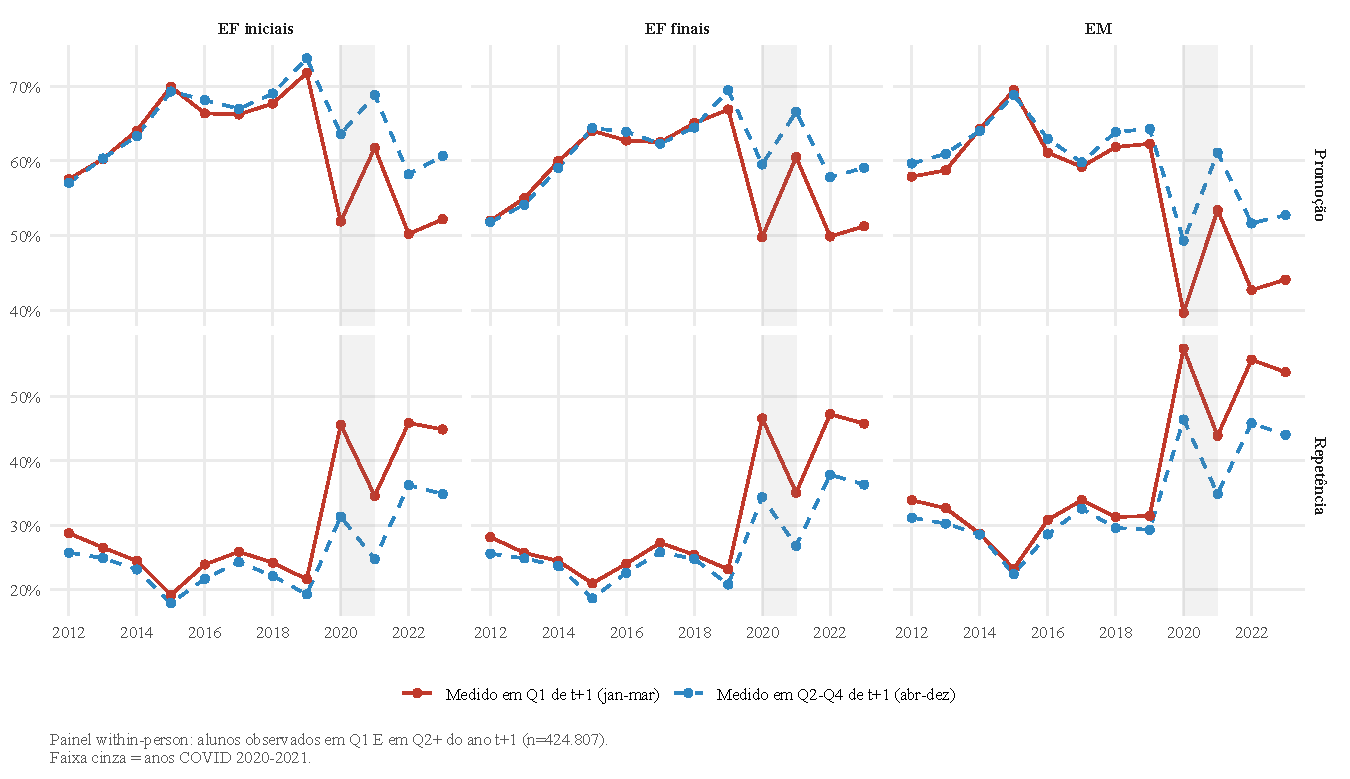
\includegraphics[width=0.95\textwidth]{../DataWork/5_Figures/output/F6_efeito_ferias_within.pdf}
\caption{Efeito do timing da observação de $t+1$ sobre promoção e
repetência (painel \emph{within-person}), por macroetapa.}
\label{fig:efeito_ferias}
\figurenote{Subamostra de alunos com observação em $Q_1$ e em algum
$Q \geq 2$ de $t+1$. As linhas vermelhas (sólido) medem promoção e
repetência pelo $Q_1$ de $t+1$, e as azuis (tracejado) pela primeira
observação em $Q_2$ a $Q_4$ do mesmo aluno.}
\end{figure}

A escolha da janela do indicador intra-ano foi testada em duas
variantes, a saber, primeira observação no ano $t$ contra última
observação no ano $t$, e visita $V_1$ contra visita $V_5$ por
indivíduo, e ambas produzem resultados estáveis. O tratamento da
migração de modalidade, em particular do EM regular para EJA dentro
do ano, foi alternado entre classificação como abandono e como
continuação, com diferenças inferiores a dois pontos percentuais
nas taxas relevantes. A idade-padrão para defasagem foi alternada
entre entrada aos seis anos e entrada aos sete anos no primeiro ano
do EF, sem alteração qualitativa dos resultados. As estimativas
principais da Tabela~\ref{tab:t1_brasil} são, em suma, estáveis a
essas variações, com diferenças menores que dois pontos
percentuais.

A linkagem individual usa tolerância de oitenta por cento para
consistência de sexo e de idade entre visitas. Como sensibilidade,
testamos duas variantes. Na variante \emph{strict}, exigimos cem
por cento de consistência, o que é mais conservador; na variante
\emph{loose}, aceitamos sessenta por cento de consistência,
recuperando mais indivíduos. A reponderação dos indicadores
principais sob essas variantes não move nenhum indicador além de
1,5 pontos percentuais, o que confirma a estabilidade do algoritmo
central. Para aproximadamente vinte por cento das transições
inter-ano, dispomos da Visita 5 da PNADC anual com a variável
\texttt{V5002A}, que indica recebimento de Bolsa Família. Nessa
subamostra, comparamos o perfil de fluxo dos indivíduos com BFA
observado contra os com perfil de renda compatível, mas sem BFA
observado. Os detalhes desta comparação serão preenchidos quando o
módulo B4 da estimação estiver completo.

A identidade contábil Promoção mais Repetência mais Evasão mais
Migração EJA igual a um deve ser aproximadamente satisfeita por
construção. Sob a metodologia v5, com a correção \texttt{V3014}
incorporada, a soma fica em torno de 98\% no EF iniciais e finais
e 97\% no EM. O resíduo de aproximadamente 2 a 3\% é atribuível a
transições para ensino superior, modalidades não classificadas e
casos limítrofes de matrícula em redes não cobertas pelo
\texttt{V3002A}. A PNADC mudou a codificação da
variável \texttt{V3003} em 2016, substituindo-a por \texttt{V3003A}
com códigos diferentes. A harmonização descrita no
Apêndice~\ref{app:variaveis} reconcilia os dois períodos. Para
validar, comparamos os indicadores das transições 2013/2014 e
2014/2015, pré-mudança, com 2016/2017 e 2017/2018, pós-mudança.
As séries são contínuas, sem descontinuidades visíveis na
Figura~\ref{fig:cohort_fluxo}, o que confirma que a harmonização
foi bem-sucedida.
